\section{Blockchain-based Marketplace Trading Schemes }
\label{sec:blockchain-marketplace-trading-schemes}

This section presents three papers related to marketplace data trading using blockchain in different domains.
The first and third papers address medical domain applications, while the second paper targets an IoT domain application.
The papers are presented in chronological order, from most recent to oldest.

\subsection{Blockchain-based Fair and Fine-grained Data Trading with Privacy Preservation~\cite{xue2023blockchain}}
\label{sec:blockchain-based-medical-data-marketplace-23}

\subsubsection{Problem Definition and Network Model}
\label{sec:2023-problem-definition}
In healthcare data trading, an EMR contains much personal information about the patient, such as her name, age, and address.
EMR records have to be signed by a hospital to guarantee fair trading.
A data buyer who can be a pharmaceutical company, for example, submits a smart contract to the marketplace that it is interested to buy EMR reports from patients (data sellers) who satisfy certain conditions, and it is interested only in a specific set of attributes.
An example EMR report is shown in \cref{fig:example-emr-report}.
The data buyer may be interested in \textbf{Diastolic Blood Pressure, Glucose, and Serum Insuline} attributes only for patients whose Diagnosis is Diabetes only.
During the trading process, the identity of both the hospitals and the data sellers is hidden from the data buyer.
The network model comprises five entities: HD, hospitals, data sellers, and data buyers, as shown in \cref{fig:network_model}.
HD generates public system parameters.

\begin{figure}
\centering
  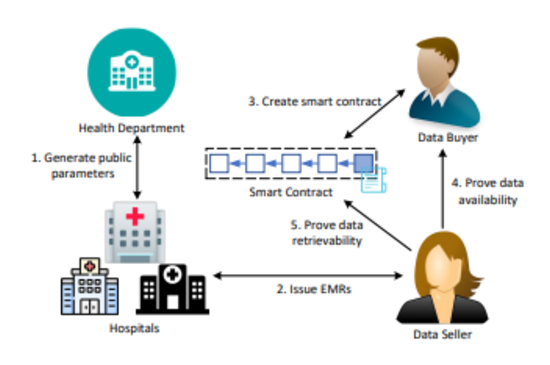
\includegraphics[width=0.96\linewidth]{imgs/23-network-model.eps}
  \caption{Network model~\cite{xue2023blockchain}}
  \label{fig:network_model}
  %\vspace{-5mm}
\end{figure}

\begin{figure}
\centering
  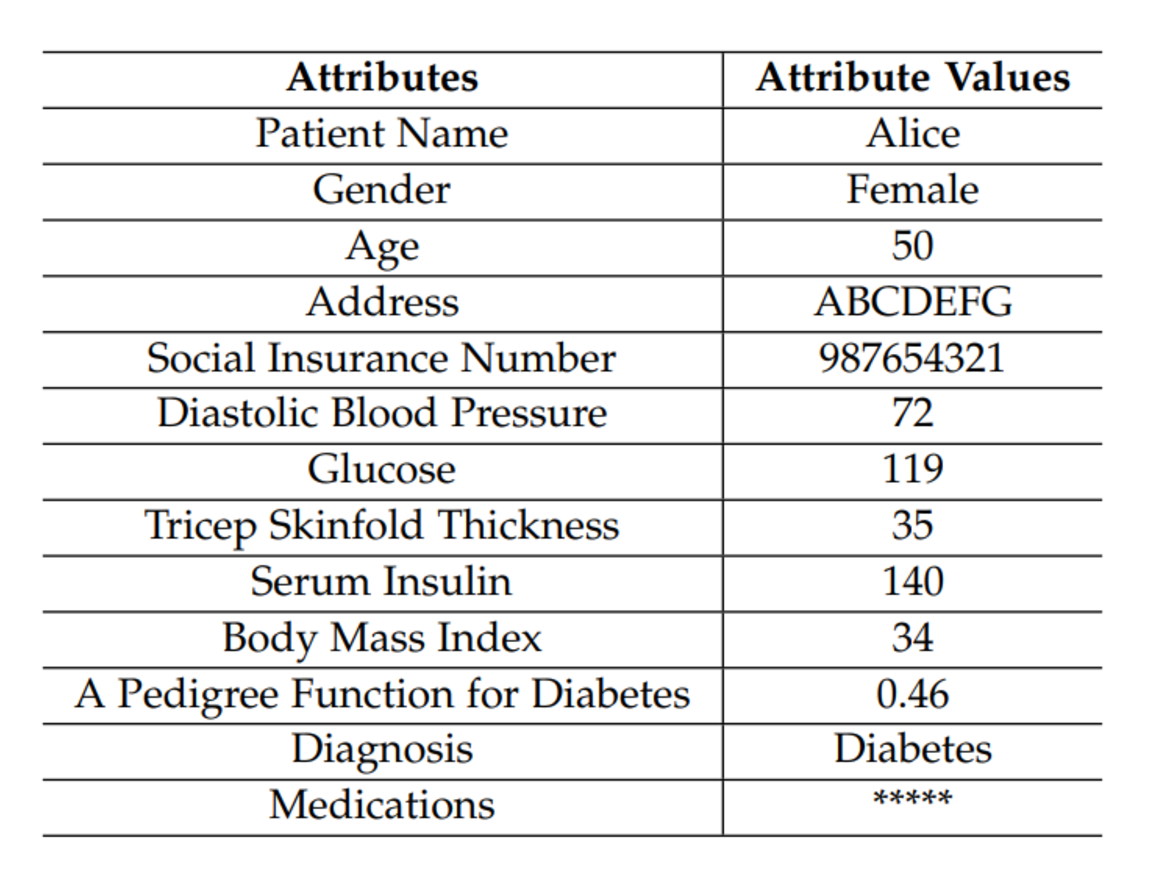
\includegraphics[width=0.8\linewidth]{imgs/23-example-emr-report.eps}
  \caption{An example EMR report~\cite{xue2023blockchain}}
  \label{fig:example-emr-report}
  %\vspace{-5mm}
\end{figure}

\subsubsection{Contributions}
The contributions of this paper are as follows:
\begin{itemize}
    \item Present a strategy for the data seller to sell the EMR report in parts (individual attributes), without affecting the ability of their verification
    \item Data fields attributes are signed by the hospital to ensure the integrity of the EMR reports while hiding the real identity of the hospital from the data buyer
\end{itemize}

\subsubsection{Threat Model}
In this paper, HD and hospitals are honest.
Data sellers and buyers can be malicious, as for data sellers, they want to gain as much money from data buyers as they could.
On the other hand, data buyers want to get access to the EMR reports without paying or get access to private information about the patients or the hospitals that they are not supposed to have access to.

\subsubsection{Used Schemes}
The paper uses the following building blocks:

\begin{itemize}
    \item \textbf{Structure-preserving Signature}~\cite{gay2018more}: A signature scheme that offers signature randomization and proved to be efficient in verification. That is why it is used in blockchain applications
    \item \textbf{ZKP}: This scheme is used to prove knowledge of correct encryption of the EMR report by the seller without revealing the encryption secret key to the buyer
    \item \textbf{Merkle Hash Tree}: This structure is used to hash the attributes inside an EMR report to prove that the attributes are related to the same report
    \item \textbf{AES}: This scheme is used to encrypt the attributes with a symmetric key $k$
    \item \textbf{El-gamal Encryption}: This scheme is used to encrypt the symmetric key $k$ using the buyer's public key
\end{itemize}

\subsubsection{Solution Overview}

In this section, the steps solution suggested in the paper is summarized, as shown in~\cref{fig:23-interactions-through-smart-contract} and following the example presented in \cref{sec:2023-problem-definition}:

\begin{itemize}
    \item \textbf{Policy Definition}: If the data buyer wants to gather EMR reports related to diabetes, then a smart contract will be initiated by him stating the requirements in terms of mandatory attribute values in the report and the attributes required to be gathered from the seller and signs them. In this case, the attribute value \textit{Disease} shall have the value \textit{diabetes}, and the attribute required to be collected from the users are: \textit{Glucose, Diastolic Blood Pressure, Serum Insulin, and Age}. In addition, he deposits the data reward to the smart contract
    \item \textbf{Policy Verification}: If the data seller has the required attributes, she verifies the signature on the required attributes using the buyer's public key
    \item \textbf{Present}: The data seller proves that she has the required data by sending the signature on the attributes, the ciphertext of the attribute values $CB$, and a ZKP of the correct encryption
    \item The smart contract checks the proof that the data seller has the required legitimate attributes, as posted by the data seller. Then it sends a notification to the data buyer, who will recheck the proof and that the data seller meets the requirements posted in the definition of the policy, then he sends a confirmation message $CM$ to the smart contract
    \item \textbf{Ciphertext Generation}: The data seller encrypts the attributes encryption key $k$ with the buyer's public key $bpk$ to form the ciphertext $CK`$. She sends the ciphertext with the ZKP of the correct encryption $\pi_b$ to the smart contract
    \item \textbf{Ciphertext Retrieval}: The smart contract checks the validity of the proof and sends a notification to the data buyer. Afterward, The data buyer retrieves the ciphertext key and decrypts $CB$ to get the attribute values required
\end{itemize}

\begin{figure}
\centering
  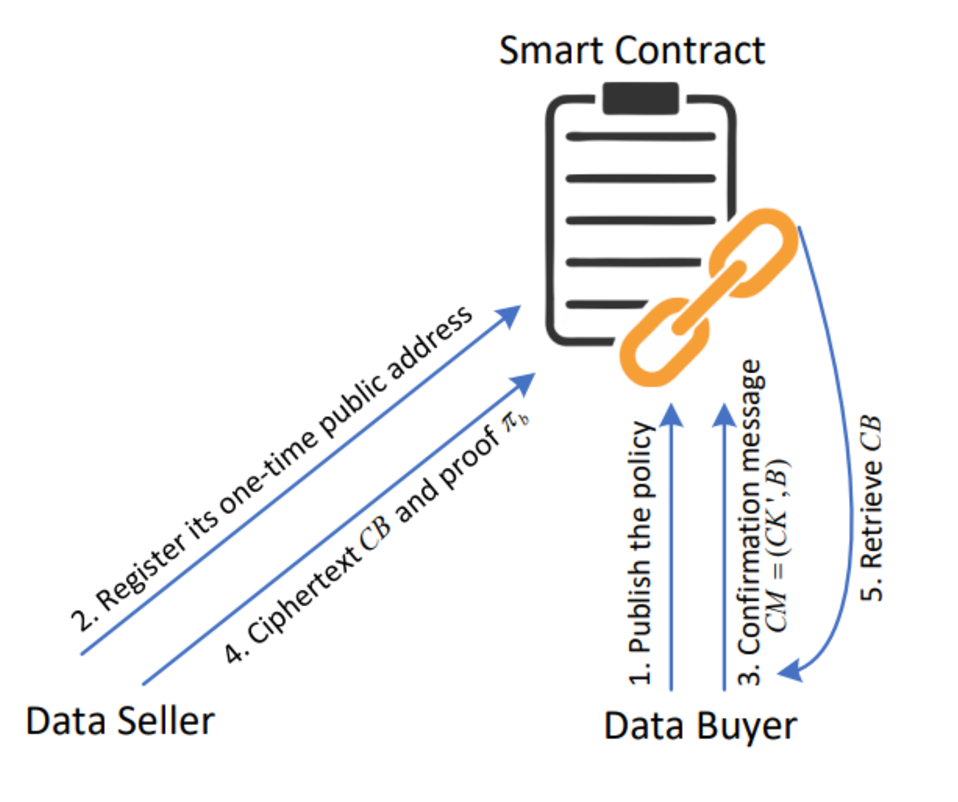
\includegraphics[width=0.8\linewidth]{imgs/23-interactions.eps}
  \caption{Interactions through the smart contract~\cite{xue2023blockchain}}
  \label{fig:23-interactions-through-smart-contract}
  %\vspace{-5mm}
\end{figure}

\subsection{Blockchain-cloud transparent data marketing: Consortium management and fairness~\cite{liu2022blockchain}}
\label{sec:blockchain-cloud-trasparent-data-marketing-consortium-management}

\subsubsection{Problem Definition and Network Model}

\subsubsection{Contributions}

\subsubsection{Threat Model}

\subsubsection{Used Schemes}

\subsubsection{Solution Overview}

\subsection{A Blockchain-based Medical Data Marketplace with Trustless Fair Exchange and Access~\cite{alsharif2020blockchain}}
\label{sec:blockchain-based-medical-data-marketplace-20}

\subsubsection{Problem Definition and Network Model}

\subsubsection{Contributions}

\subsubsection{Threat Model}

\subsubsection{Used Schemes}

\subsubsection{Solution Overview}
